\documentclass{standalone}

% Packages
	% Basics
		\usepackage{amsmath}
		\usepackage{amssymb}
		\usepackage{bm}
		\usepackage[utf8]{inputenc}
	% Diagrams
		\usepackage{pgfplots}
		\usepackage{tikz}
		\usepackage{tikz-3dplot}
			\usetikzlibrary{arrows,decorations.markings,plotmarks}

\begin{document}
	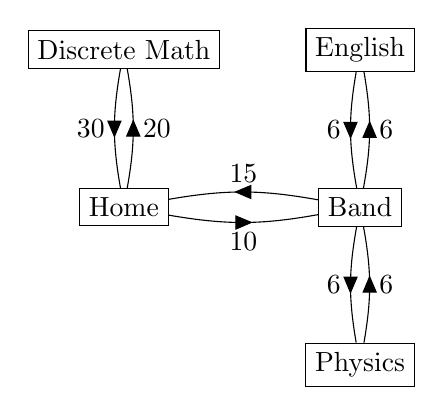
\begin{tikzpicture}[
		    midarr/.style 2 args={
		        decoration={             
		            markings, 
		            mark=at position 0.5 with {\arrow[xshift=3.333pt]{triangle 45}, \node[#1] {#2};}
		        },
		        postaction={decorate}
			}
		]
		\node[draw] (Home) at (0, 0) {Home};
		\node[draw] (Band) at (3, 0) {Band};
		\node[draw] (English) at (3, 2) {English};
		\node[draw] (Physics) at (3, -2) {Physics};
		\node[draw] (Discrete Math) at (0, 2) {Discrete Math};
		\draw[midarr] (Home) to[bend right = 10] node[below]{10} (Band);
		\draw[midarr] (Band) to[bend right = 10] node[right]{6} (English);
		\draw[midarr] (English) to[bend right = 10] node[left]{6} (Band);
		\draw[midarr] (Band) to[bend right = 10] node[left]{6} (Physics);
		\draw[midarr] (Physics) to[bend right = 10] node[right]{6} (Band);
		\draw[midarr] (Band) to[bend right = 10] node[above]{15} (Home);
		\draw[midarr] (Home) to[bend right = 10] node[right]{20} (Discrete Math);
		\draw[midarr] (Discrete Math) to[bend right = 10] node[left]{30} (Home);
	\end{tikzpicture}	
\end{document}
